

\chapter{Resultados}

Texto texto texto texto texto texto texto texto texto texto texto texto texto texto texto texto texto texto texto texto texto texto texto texto texto texto texto texto texto texto texto texto texto texto texto texto texto texto texto texto texto texto texto texto.

\begin{figure}[htb]
	\caption{\label{fig_grafico}Gráfico produzido em Excel e salvo como PDF}
	\begin{center}
	    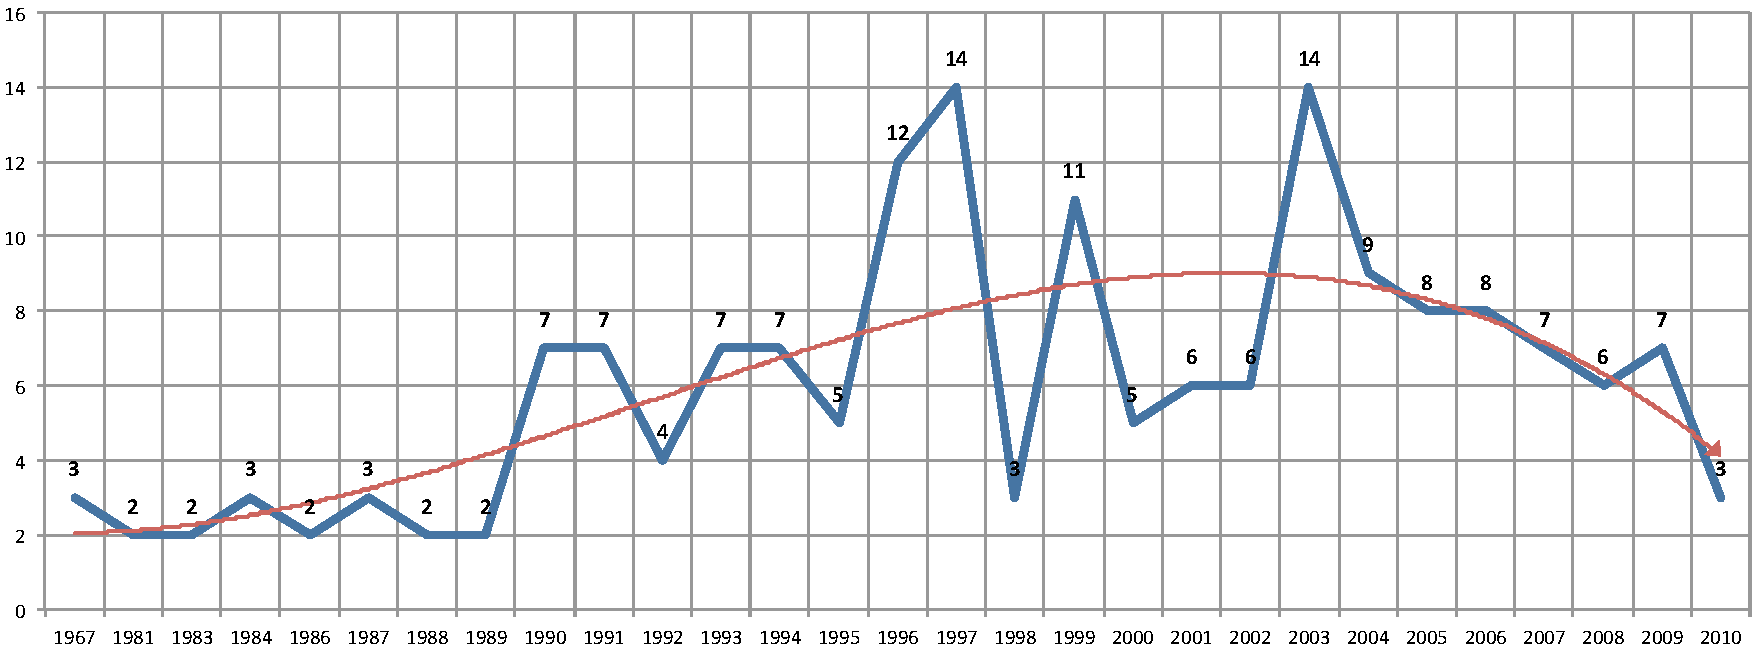
\includegraphics[scale=0.5]{imagens/abntex2-modelo-img-grafico.pdf}
	\end{center}
	\legend{Fonte: \citeonline[p. 24]{araujo2012}}
\end{figure}



\emph{Minipages} são usadas para inserir textos ou outros elementos em quadros
com tamanhos e posições controladas. Veja o exemplo da
\autoref{fig_minipage_imagem1} e da \autoref{fig_minipage_grafico2}.

\begin{figure}[htb]
 \label{teste}
 \centering
  \begin{minipage}{0.4\textwidth}
    \centering
    \caption{Imagem 1 da minipage} \label{fig_minipage_imagem1}
    
\includegraphics[scale=0.2]{imagens/ifpi.pdf}
    \legend{Fonte: Produzido pelos autores}
  \end{minipage}
  \hfill
  \begin{minipage}{0.4\textwidth}
    \centering
    \caption{Grafico 2 da minipage} \label{fig_minipage_grafico2}
    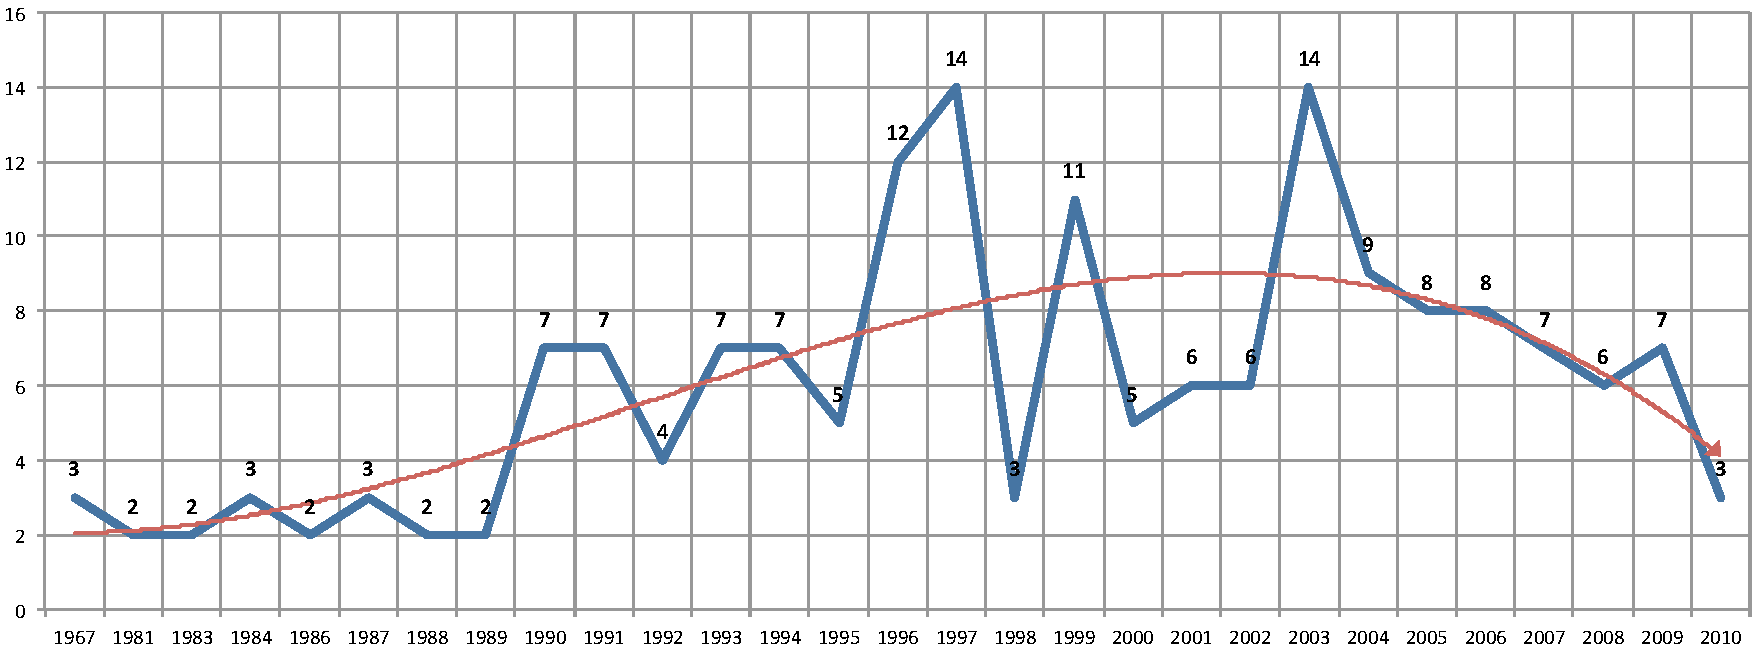
\includegraphics[scale=0.2]{imagens/abntex2-modelo-img-grafico.pdf}
    \legend{Fonte: \citeonline[p. 24]{araujo2012}}
  \end{minipage}
\end{figure}

Observe que, segundo a \citeonline[seções 4.2.1.10 e 5.8]{NBR14724:2011}, as
ilustrações devem sempre ter numeração contínua e única em todo o documento.

\begin{citacao}
Qualquer que seja o tipo de ilustração, sua identificação aparece na parte
superior, precedida da palavra designativa (desenho, esquema, fluxograma,
fotografia, gráfico, mapa, organograma, planta, quadro, retrato, figura,
imagem, entre outros), seguida de seu número de ordem de ocorrência no texto,
em algarismos arábicos, travessão e do respectivo título. Após a ilustração, na
parte inferior, indicar a fonte consultada (elemento obrigatório, mesmo que
seja produção do próprio autor), legenda, notas e outras informações
necessárias à sua compreensão (se houver). A ilustração deve ser citada no
texto e inserida o mais próximo possível do trecho a que se
refere. \cite[seções 5.8]{NBR14724:2011}
\end{citacao}



